%This is my super simple Real Analysis Homework template

\documentclass{article}

%% Language and font encodings
\usepackage[T1,T8K,T8M]{fontenc}
\usepackage[utf8]{inputenc}
\usepackage[english,georgian]{babel}

\usepackage{amsmath}
\usepackage{graphicx}
\usepackage[colorinlistoftodos]{todonotes}
\usepackage[colorlinks=true, allcolors=blue]{hyperref}
\usepackage{float}
\usepackage{enumerate}
\usepackage{subfig}
\usepackage{gensymb}

%\title{დავალება 01}
%\author{Your Name}
%\date\today
%This information doesn't actually show up on your document unless you use the maketitle command below

\begin{document}

\subsection{ამოცანა 1}
%კურკუმული გვერდი 149
სამი ერთნაირი მილი (თითოეული $P$ წონით) მოთავსებულია ისე, როგორც ნახაზზეა ნაჩვენები \ref{fig:01}. განსაზღვრეთ ქვედა მილების რეაქციის ძალა დედამიწაზე და კედლებზე.
	\begin{figure}[H]
		\centering
		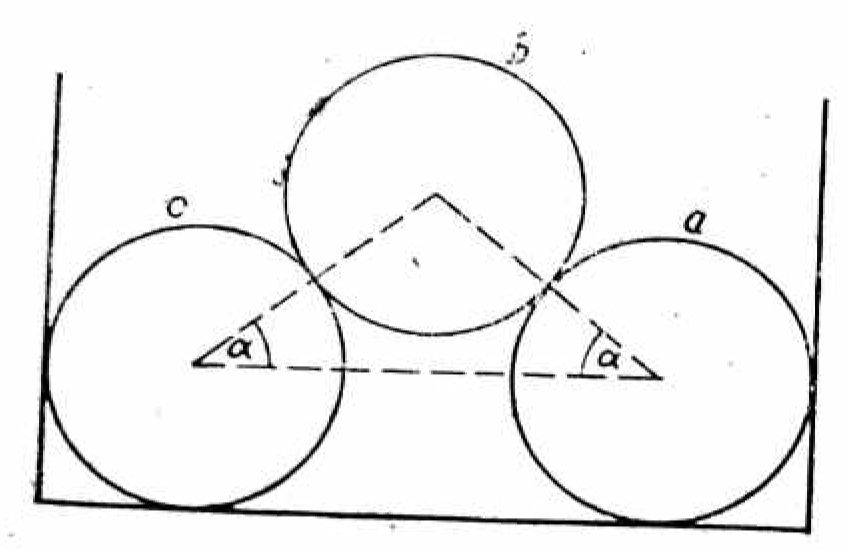
\includegraphics[width=0.2\columnwidth]{figures/01}
		\caption{პირველი ამოცანა.}
		\label{fig:01}
		\end{figure}
		
\subsection{ამოცანა 2}
%კურკუმული 141
$m$ მასის და $l$ სიგრძის კიბე მიდგმულია კედელთან $\alpha$ კუთხით. ადამიანი გარეთ ეწევა კიბეს ჰორიზონტალური მიმართელებით (ძალა კიბის შუაშია მოდებული). იმ ძალის უმცირესი მნიშვნელობა, რომლის დროსაც კიბის ზედა ბოლო მოშორდება კედელს არის $F$. იატაკიდან რა სიმაღლეზეა მოთავსებული კიბის სიმძიმის ცენტრი?

\subsection{ამოცანა 3}
%გედენიძე 1071
გლუვ შვეულ კედელზე მიყუდებული $m$ მასის კიბე ჰორიზონტალურ ზედაპირთან $\alpha$ კუთხეს ქმნის. კიბის მასათა ცენტრი მის შუაშია. განსაზღვრეთ და სურათზე გამოსახეთ კიბეზე მოქმედი ძალები.

\subsection{ამოცანა 4}
%გედენიძე 1072
კიბე, რომლის მასათა ცენტრი მის შუაშია. შვეულ კედელსა და მიწას ეყრდნობა. კედელთან ხახუნის კოეფიციენტი $\mu_1 = 0.4$-ია, მიწასთან - $\mu_2 = 0.5$. რა მინიმალურ კუთხეს უნდა ქმნიდეს კიბე ჰორიზონტალურ ზედაპირთან, რომ არ მოცურდეს?


\subsection{ამოცანა 5}
%გედენიძე 1073
3მ სიგრძის მსუბუქი კიბე ეყრდნობა გლუვ შვეულ კედელს და მასთან $60 \degree$-იან კუთხეს ქმნის ჰორიზონტალურ საყრდენთან ხახუნის ძალა 300ნ-ია. რა სიმაღლეზე შეძლებს 70კგ მასის კაცი ასვლას, კიბე რომ არ მოცურდეს?

\end{document}